\section{Stabilność wzorców uczących}
\label{sec:stabilnosc}

Rozdział sprawdza, które wzorce uczące są punktami stałymi sieci po uczeniu każdą z reguł, i wyjaśnia, dlaczego reguła Hebba zawodzi na dostarczonych zbiorach. Wykorzystano eksperymenty \texttt{stability}, \texttt{stability-single-neuron}, \texttt{capacity} i \texttt{large-recovery} z Tabeli~\ref{tab:eksperymenty}.

\subsection{Stabilne wzorce}
\label{sec:stabilne-wzorce}

Liczby stabilnych wzorców w ośmiu dostarczonych zbiorach podano w Tabeli~\ref{tab:stabilne}. Wzorzec jest stabilny, gdy żaden jego piksel nie ma ujemnego pola wyrównanego $\xi^\mu_i h_i$ (rozdział~\ref{sec:metryki}). Taki wzorzec jest punktem stałym w obu trybach dynamiki, więc wynik nie zależy od trybu.

\begin{table}[H]
    \centering
    \caption{Stabilne wzorce po uczeniu trzema regułami. Kolumna \enquote{niestabilne piksele} podaje łączną liczbę pikseli z ujemnym polem wyrównanym we wszystkich wzorcach zbioru przy regule Hebba. Ostatnia kolumna podaje liczbę wzorców spełniających warunek wystarczający $\sum_{\nu \ne \mu} \lvert m^{\mu\nu} \rvert < 1 - p/N$.}
    \label{tab:stabilne}
    \small
    \begin{tabular}{l r r r r r r}
        \toprule
        & & \multicolumn{3}{c}{stabilne wzorce} & niestabilne & \\
        \cmidrule(lr){3-5}
        Zbiór & $p/N$ & Hebb & Oja podprz. & Oja jednoneur. & piksele (Hebb) & warunek \\
        \midrule
        \texttt{small-7x7} & \num{0.102} & 3/5 & 5/5 & 0/5 & 7 & 1/5 \\
        \texttt{letters-abc-8x12} & \num{0.031} & 0/3 & 3/3 & 0/3 & 14 & 0/3 \\
        \texttt{animals-14x9} & \num{0.048} & 2/6 & 6/6 & 0/6 & 24 & 2/6 \\
        \texttt{letters-14x20} & \num{0.093} & 0/26 & 26/26 & 0/26 & 590 & 0/26 \\
        \texttt{OCRA-12x30-cut} & \num{0.019} & 1/7 & 7/7 & 0/7 & 147 & 1/7 \\
        \texttt{large-25x25} & \num{0.010} & 5/6 & 6/6 & 0/6 & 30 & 5/6 \\
        \texttt{large-25x25.plus} & \num{0.024} & 1/15 & 15/15 & 0/15 & \num{1067} & 1/15 \\
        \texttt{large-25x50} & \num{0.005} & 0/6 & 6/6 & 0/6 & 700 & 0/6 \\
        \bottomrule
    \end{tabular}
\end{table}

\noindent Reguła Oji w wariancie podprzestrzeni stabilizuje wszystkie wzorce we wszystkich zbiorach. Najmniejsze pole wyrównane wynosi od \num{0.387} (\texttt{letters-14x20}) do \num{0.983} (\texttt{large-25x50}) i jest zawsze dodatnie, zgodnie z $h_i = (1 - P_{ii}) \xi^\mu_i$ z rozdziału~\ref{sec:regula-oji}. Uczenie trwało od 128 do 538 epok, z wyjątkiem \texttt{letters-14x20}, który wymagał \num{70371} epok. Zgodnie z~\eqref{eq:oja-epoka} tempo zbieżności kierunku własnego jest proporcjonalne do $\eta \lambda_k / p$. Najmniejsza wartość własna macierzy nakładań liter wynosi $\num{0.0023}$, co daje $\eta \lambda_k / p \approx \num{4.3e-5}$, podczas gdy w pozostałych zbiorach ta wielkość wynosi co najmniej \num{0.013}.

Wariant jednoneuronowy nie stabilizuje żadnego wzorca. W każdym zbiorze wszystkie wzorce przechodzą w jednym kroku do stanu pozornego o tej samej energii. Zgadza się to z wnioskiem z rozdziału~\ref{sec:regula-oji}, że przy macierzy rzędu 1 stabilne mogą być tylko stany $\pm \operatorname{sgn}(c_1)$.

Reguła Hebba stabilizuje łącznie 12 z 74 wzorców, a większość wzorców zbioru tylko w \texttt{large-25x25} i \texttt{small-7x7}. Niestabilne wzorce podane na wejście kończą w stanach pozornych, a tylko w \texttt{small-7x7} jeden z nich przechodzi w negację innego wzorca. Wszystkie 26 liter \texttt{letters-14x20} trafia do tego samego stanu pozornego, najbardziej podobnego do litery r ($m = \num{0.929}$).

\subsection{Dlaczego reguła Hebba zawodzi}
\label{sec:dlaczego-hebb}

Według rozkładu~\eqref{eq:przesluch} wzorzec jest stabilny, gdy składnik zakłócający nie zmienia znaku pola w żadnym pikselu. Warunek wystarczający spełnia tylko 10 z 74 wzorców (Tabela~\ref{tab:stabilne}). Warunek nie jest konieczny, ale wzorce, które go nie spełniają, są stabilne tylko wyjątkowo.

Najwyraźniej widać to na literach. Litera zajmuje niewielką część bitmapy, więc dwie różne litery zgadzają się w większości pikseli wspólnego białego tła. Wszystkie nakładania w \texttt{letters-14x20} są dodatnie (co najmniej \num{0.486}), a ich suma dla jednego wzorca wynosi od \num{14.9} do \num{19.8}, czyli kilkanaście razy więcej niż sygnał $1 - p/N \approx \num{0.91}$. Przy dodatnich nakładaniach składnik zakłócający $\sum_{\mu \ne \nu} \xi^\mu_i m^{\mu\nu}$ działa jak ważone głosowanie pozostałych liter i przeważa sygnał. Niestabilne mogą być więc tylko piksele, w których litera różni się od większości pozostałych. Niestabilne piksele wszystkich liter pokazano na Rysunku~\ref{fig:niestabilne-litery}. Każdy z 590 niestabilnych pikseli jest pikselem, w którym litera różni się od większości pozostałych 25 liter, a wszystkich takich pikseli jest 778.

\begin{figure}[H]
    \centering
    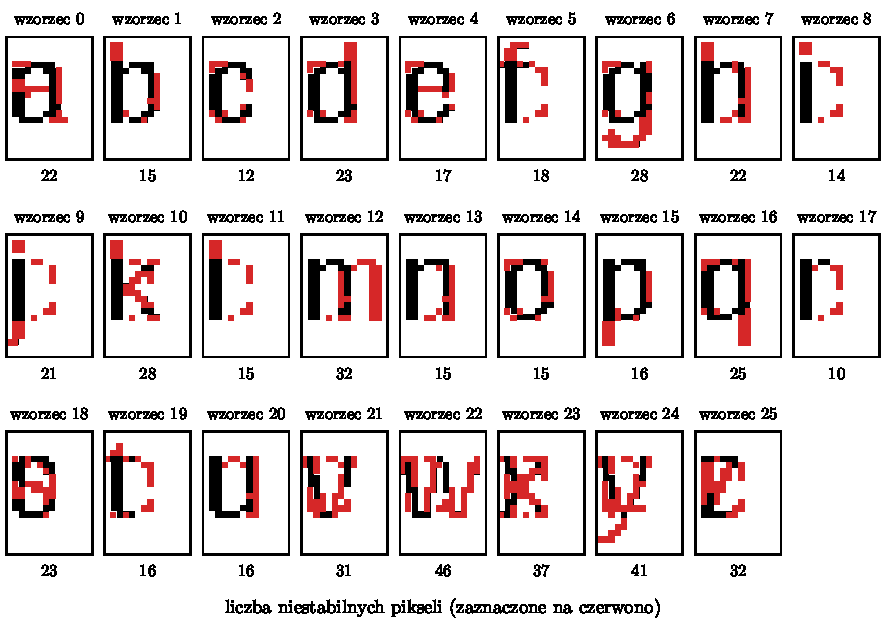
\includegraphics[width=0.75\textwidth]{08-stability/figures/unstable-letters-14x20.pdf}
    \caption{Niestabilne piksele liter \texttt{letters-14x20} przy regule Hebba (zaznaczone na czerwono). Pod każdą literą podano liczbę jej niestabilnych pikseli.}
    \label{fig:niestabilne-litery}
\end{figure}

\noindent Wpływ korelacji wzorców widać też w eksperymencie \texttt{capacity}, w którym stabilność sprawdzono dla rosnącej liczby wzorców (Rysunek~\ref{fig:pojemnosc}). Dla wzorców losowych odsetek stabilnych wzorców przy regule Hebba zgadza się z przybliżeniem $(1 - P_\text{bit})^N$ wynikającym z~\eqref{eq:p-bit}, a dane leżą nieco powyżej teorii, na przykład dla $N = 280$ i $p = 40$ wynoszą \num{0.442} wobec \num{0.319}. Wszystkie 50 zbiorów losowych jest w pełni stabilnych do $p = 12$ przy $N = 280$ i do $p = 25$ przy $N = 625$, czyli do $p/N \approx \num{0.04}$. Zbiory dostarczone tracą stabilność przy obciążeniu kilka razy mniejszym. W \texttt{letters-14x20} już od $p = 3$ ($p/N = \num{0.011}$) żaden wzorzec nie jest stabilny, podczas gdy losowe zbiory o tym samym $N$ i $p = 26$ mają średnio \num{0.898} stabilnych wzorców. W \texttt{large-25x25.plus} wszystkie wzorce są stabilne do $p = 5$. Reguła Oji stabilizuje wszystkie wzorce we wszystkich \num{3541} zbiorach tego eksperymentu.

\begin{figure}[H]
    \centering
    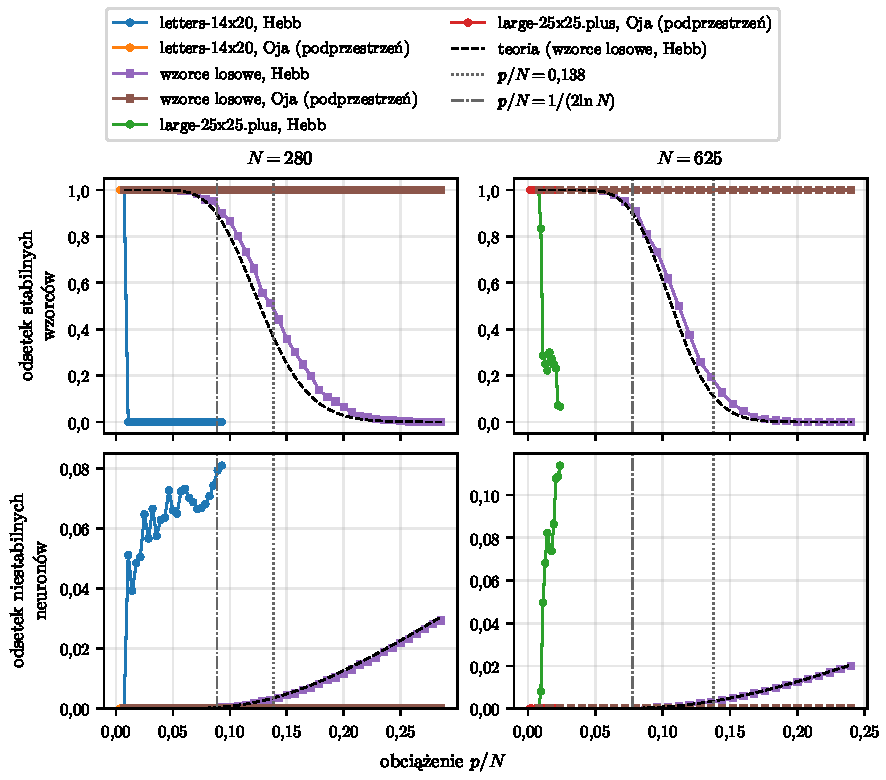
\includegraphics[width=0.7\textwidth]{08-capacity/figures/capacity.pdf}
    \caption{Stabilność wzorców w funkcji obciążenia $p/N$ dla $N = 280$ (lewa kolumna) i $N = 625$ (prawa kolumna). Wzorce losowe to średnia z 50 zbiorów na każde $p$, a zbiory dostarczone to ich początkowe fragmenty o $p$ wzorcach. Górne wykresy: średni odsetek stabilnych wzorców. Dolne wykresy: odsetek niestabilnych neuronów. Linia przerywana to teoria~\eqref{eq:p-bit}, a pionowe linie to granice $p/N = 1/(2 \ln N)$ i $p/N = \num{0.138}$.}
    \label{fig:pojemnosc}
\end{figure}

\noindent Wyniki zgadzają się z literaturą przytoczoną w rozdziale~\ref{sec:regula-hebba}. Granice pojemności dotyczą wzorców losowych, a dla wzorców skorelowanych reguła Hebba nie gwarantuje stabilności~\cite[s.~L-364]{personnaz1985}. Podobne wzorce zlewają się w jeden stan stabilny~\cite[s.~2557]{hopfield1982}, co na literach prowadzi do jednego wspólnego stanu pozornego.

\subsection{Zbiory 25x25 i 25x50}
\label{sec:zbiory-25x50}

Zbiory \texttt{large-25x25} i \texttt{large-25x50} zawierają te same sześć obrazów. W drugim z nich każdy obraz dopełniono dolną połową złożoną z 625 pikseli $+1$, wspólną dla wszystkich wzorców. Dopełnienie dodaje do sumy w~\eqref{eq:nakladanie} 625 zgodnych pikseli przy dwukrotnie większym $N$, więc
\begin{equation}
    m^{\mu\nu}_{25 \times 50} = \frac{m^{\mu\nu}_{25 \times 25} + 1}{2}.
    \label{eq:nakladanie-25x50}
\end{equation}
Nakładania obu zbiorów pokazano na Rysunku~\ref{fig:nakladania-25x50}. Pary prawie ortogonalne w \texttt{large-25x25} mają w \texttt{large-25x50} nakładanie około \num{0.5}, a średnie $\lvert m \rvert$ rośnie z \num{0.142} do \num{0.567}. Suma $\sum_{\nu \ne \mu} \lvert m^{\mu\nu} \rvert$ rośnie z zakresu \numrange{0.056}{1.118} do \numrange{2.475}{3.042}, więc żaden wzorzec nie spełnia warunku wystarczającego. Mniejsze obciążenie $p/N$ (\num{0.005} wobec \num{0.010}) nie pomaga, bo składnik zakłócający w~\eqref{eq:przesluch} zależy od nakładań, a nie od $N$. W efekcie reguła Hebba stabilizuje 5 z 6 wzorców \texttt{large-25x25} i żadnego wzorca \texttt{large-25x50}, a liczba niestabilnych pikseli rośnie z 30 do 700.

\begin{figure}[H]
    \centering
    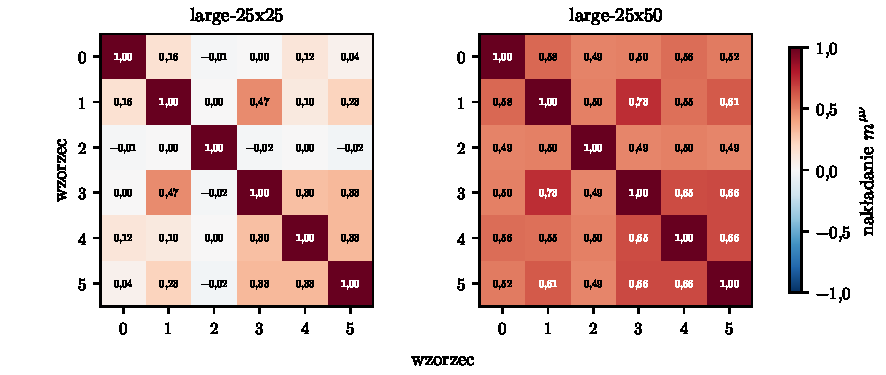
\includegraphics[width=0.8\textwidth]{08-stability/figures/overlaps-large.pdf}
    \caption{Nakładania $m^{\mu\nu}$ par wzorców w zbiorach \texttt{large-25x25} (lewy wykres) i \texttt{large-25x50} (prawy wykres). Wartości po prawej stronie spełniają~\eqref{eq:nakladanie-25x50}.}
    \label{fig:nakladania-25x50}
\end{figure}

\noindent Różnica przenosi się na odzyskiwanie wzorców z uszkodzonego wejścia (Rysunek~\ref{fig:odzyskiwanie-large}). Przy regule Hebba sieć odzyskuje bez szumu 5 z 6 wzorców \texttt{large-25x25}, a przy rosnącym szumie coraz mniej, a w \texttt{large-25x50} nie odzyskuje żadnego wzorca na żadnym poziomie szumu, bo żaden wzorzec nie jest stabilny. Reguła Oji usuwa tę różnicę. Wszystkie trzy zbiory \texttt{large-*} są odzyskiwane w co najmniej \num{0.999} prób do szumu \num{0.35} i w co najmniej \num{0.988} prób przy szumie \num{0.4}.

\begin{figure}[H]
    \centering
    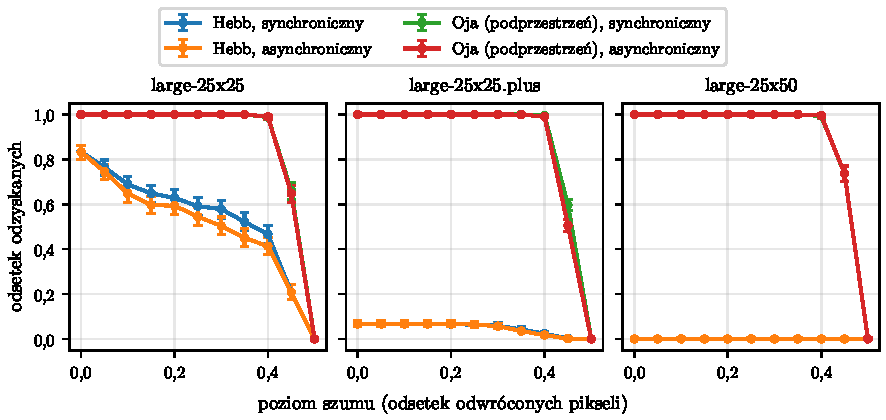
\includegraphics[width=0.9\textwidth]{08-large-recovery/figures/recovery.pdf}
    \caption{Odsetek odzyskanych wzorców w zależności od poziomu szumu dla zbiorów \texttt{large-*} (100 prób na wzorzec, słupki to 95-procentowe przedziały Wilsona). Linie obu trybów dla reguły Oji prawie się pokrywają.}
    \label{fig:odzyskiwanie-large}
\end{figure}

\subsection{Odpowiedzi na pytania}
\label{sec:stabilnosc-odpowiedzi}

\begin{enumerate}
    \item Reguła Oji w wariancie podprzestrzeni stabilizuje wszystkie 74 wzorce dostarczonych zbiorów, reguła Hebba 12 z nich, a wariant jednoneuronowy żadnego.
    \item Przy regule Oji sieć uczy się poprawnie wszystkich zbiorów. Przy regule Hebba żaden zbiór nie jest zapamiętany w całości, a większość wzorców jest stabilna tylko w \texttt{large-25x25} i \texttt{small-7x7}.
    \item Wzorce nie są stabilne, gdy suma ich nakładań z pozostałymi wzorcami jest duża w porównaniu z sygnałem. Dzieje się tak w zbiorach ze wspólnym tłem lub wspólną częścią, nawet przy małym obciążeniu $p/N$. W zbiorze liter niestabilne są wyłącznie piksele, w których litera różni się od większości pozostałych liter. Reguła Oji usuwa ten efekt, bo zbiega do rzutu na podprzestrzeń wzorców.
    \item Wspólna dolna połowa bitmap \mbox{25x50} zwiększa wszystkie nakładania zgodnie z~\eqref{eq:nakladanie-25x50}, więc przy regule Hebba żaden wzorzec nie jest stabilny i sieć nie odzyskuje żadnego wzorca. Przy regule Oji oba zbiory są odzyskiwane tak samo dobrze.
\end{enumerate}
